\documentclass[10pt]{beamer}

%%%
% PREAMBLE FOR THIS DOC 
%%%
%https://tex.stackexchange.com/questions/68821/is-it-possible-to-create-a-latex-preamble-header
\usepackage{/Users/miw267/Repos/csci246_spring2025/slides/preambles/beamer_preamble_for_CSCI246}

\usetikzlibrary{matrix}


%%% TRY TO RESHOW TOC AT EACH SECTION START (with current section highlighted)
% Reference: https://tex.stackexchange.com/questions/280436/how-to-highlight-a-specific-section-in-beamer-toc
\newcommand\tocforsect[2]{%
  \begingroup
  \edef\safesection{\thesection}
  \setcounter{section}{#1}
  \tableofcontents[#2,currentsection]
  \setcounter{section}{\safesection}
  \endgroup
}


%%%% HERES HOW TO DO IT CORRECTLY
% FIRST IN .STY FILE, DO
%\usetheme[sectionpage=none]{metropolis}
% THEN AT EACH SECTION DO
%\begin{frame}{Outline}
%  \tableofcontents[currentsection]	
%\end{frame}



%\setbeamertemplate{navigation symbols}{}
%\setbeamertemplate{footline}[frame number]{}


%%%
% DOCUMENT
%%%

\begin{document}

%\maketitle

%% Title page frame
%\begin{frame}
%    \titlepage 
%\end{frame}



\title{03/26/2025: Conditional Probability \\ \qquad \qquad \qquad \& Independence }
\author{CSCI 246: Discrete Structures}
\date{Textbook reference: Sec 32, Scheinerman}

\begin{frame}
    \titlepage 
\end{frame}


\begin{frame}
\small
\begin{mygreenbox}[title=Graded Quiz Pickup]
Quizzes are in the front of the room, grouped into four bins (A-G, H-L, M-R, S-Z) by last name. The quizzes are upside down with your last name on the back. Come find yours before, during, or after class. \\ %Only turn the quiz over if it's yours. \\ 

\textbf{Alert.} Some of you weren't here the Friday before spring break. These stacks also include uncollected reading quizzes from Wed. Mar 12 -- Intro to Probability (Part 1). 
\end{mygreenbox} 
\vfill 

\begin{myyellowbox}[title=\text{Poll}]
How many of you would like me to post the slide deck immediately after class so that you can continue working on the group exercises before the solutions are posted?
\end{myyellowbox}

\vfill 


\begin{myredbox}[title=Today's Agenda]
\begin{itemize}
	\item Reading quiz (5 mins)
	\item Mini-lecture ($\approx$ 20 mins)
	\item Group exercises ($\approx$ 20 mins)
\end{itemize}


\end{myredbox}
\vfill 

\end{frame}



\begin{frame}[standout]
Feedback on Monday's Quiz
\end{frame}

\begin{frame}{Reading Quiz}
\footnotesize 
\begin{figure}[ht]
        \centering
        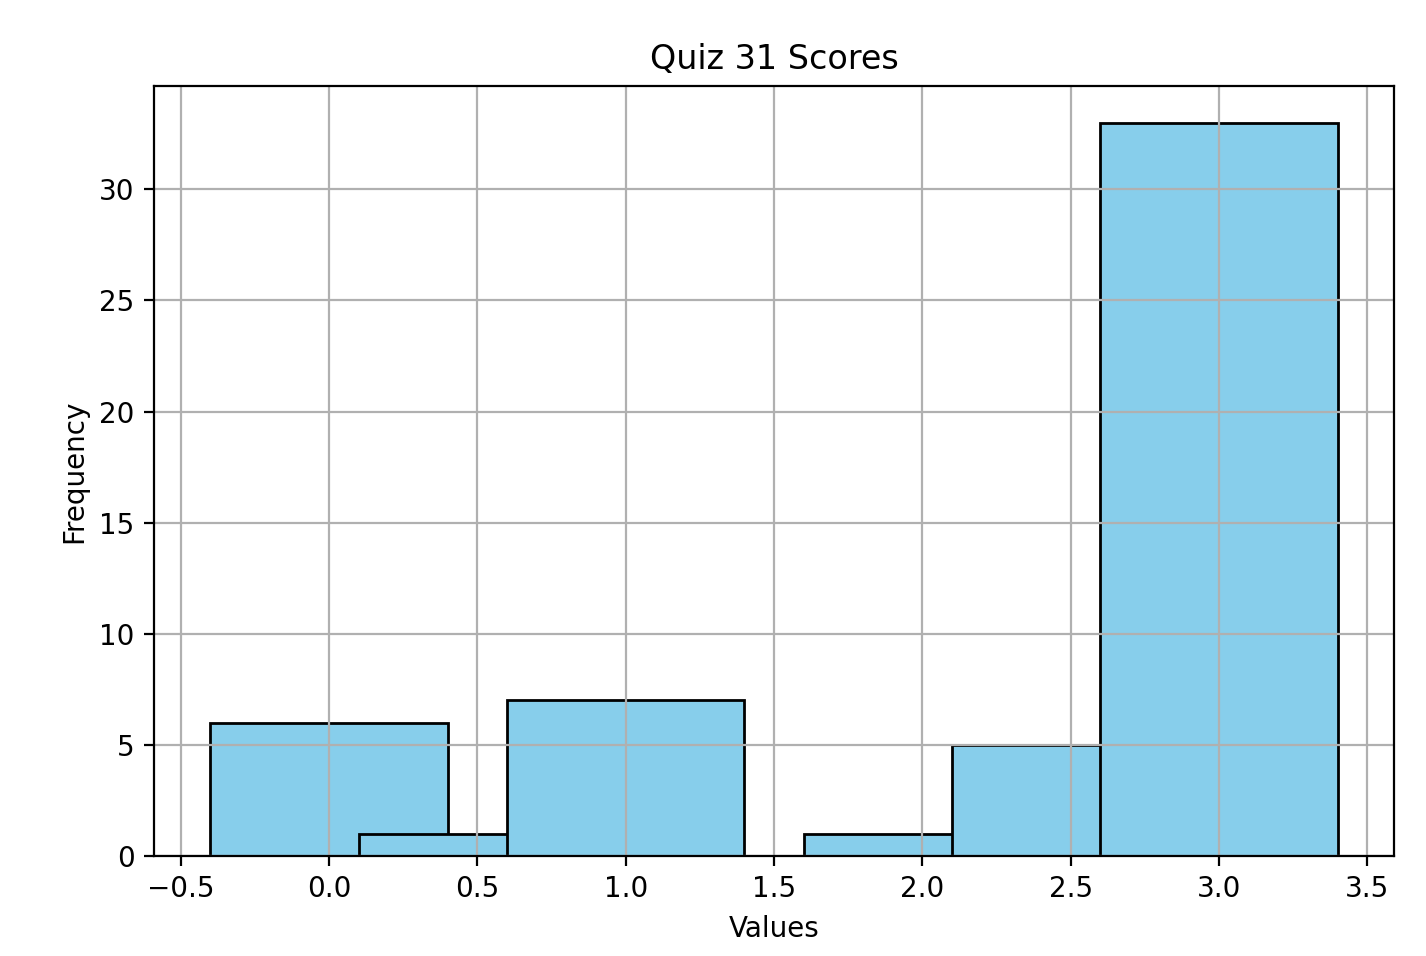
\includegraphics[width=.7\textwidth]{images/reading_quiz_scores}
   		 \caption{Median Score = 3/3 (100\%)}
\end{figure}
\vfill 
\textbf{Rubric.}  	
\begin{enumerate}
\item 1 point.  Correctly stating \textit{False}.
\item 2 points. Correctly providing fix to formula.
\end{enumerate}
\end{frame}	


\begin{frame}[standout]
Reading quiz
\end{frame}

\begin{frame}

\begin{mygreenbox}[title=\text{Reading Quiz (Conditional Probability and Independence)}]

\begin{enumerate}
\item Let $A$ and $B$ be events in a probability space $(S,P)$.   Suppose $P(B) = \frac{1}{2}$ and $P(A \cap B) = \frac{1}{8}$.  Compute $P(A \cond B)$.
\item Let $A$ and $B$ be events in a probability space $(S,P)$.  Under what condition does
\[ P(A \cap B) = P(A) P(B)?\]
\end{enumerate}

\end{mygreenbox}
	
\end{frame}


%\begin{frame}[standout]
%Introduction to Probability: \\
%Review Of Samples and Events
%\end{frame}

\begin{frame}[standout]
Review solutions to Monday's group exercises
\end{frame}


\begin{frame}[standout]
Thoughts on conditional probability and independence
\end{frame}



\begin{frame}{Conditional probability}
\footnotesize 
\begin{mygreenbox}[title=\text{Definition}]
Let $A$ and $B$ be events in a probability space $(S,P)$, and suppose $P(B) \neq 0$.  Then the \textbf{conditional probability} $ P(A \cond B)$, the probability of $A$ given $B$, is 
\[ P(A \cond B) = \frac{P(A \cap B)}{ P(B)} \]
\end{mygreenbox}

\begin{myredbox}[title=Example]

\begin{minipage}{.45\textwidth}
Let $A$ be the event of a student missing the school bus, and $B$ be the event that the student's alarm clock malfunctions. \\

Both events are rare.  But the conditional probability $P(A \cond B)$ is high.  It can be interpreted as follows: if we shrink the underlying sample space from $S$  to the event $B$, what proportion of the little black square $P(B)$ is covered by the shaded area $P(A \cap B)$? 
\end{minipage} %
\hfill 
\begin{minipage}{.45\textwidth}
\begin{figure}
\begin{center}
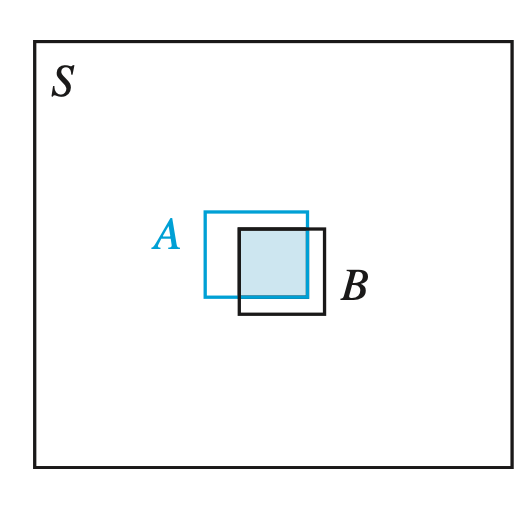
\includegraphics[width=.6\textwidth]{images/conditional_prob.png}
\end{center}
%	
\footnotesize \textbf{Figure 2:} Probability of events $A$, $B$, and $A \cap B$, given as areas. Note that the sample space $S$ must have area 1.
\end{figure}
\end{minipage} %
   
\end{myredbox}

\end{frame}


\begin{frame}

\begin{mygreenbox}[title=\text{Another interpretation of $P(A|B)$}]
If you sample an outcome from the sample space $S$ and you \textbf{know} it's in $B$, then what's the probability that it's \textbf{also} in $A$?
\end{mygreenbox}

\end{frame}



\begin{frame}
\Large 

\colorbox{red!30}{\textbf{Remark:}} \; Misunderstandings about conditional probability underly some of the most fundamental and important mistakes in human reasoning!


\end{frame}

\begin{frame}{Base rate fallacy}
\small
\colorbox{green!30}{\textbf{Example: Infectious disease test.}} Let $\mathcal{I}$ be the event that a person is infected with a disease, and $\mathcal{P}$ be the event that the person tests positive for the disease.

Suppose we collect the following data:
%
\begin{center}
\begin{tabular}{|>{\columncolor[gray]{0.85}}c|>{\columncolor[gray]{0.85}}c|>{\columncolor[gray]{0.85}}c|>{\columncolor[gray]{0.85}}c|}
\hline
\rowcolor[gray]{0.85}
\textbf{Number of people} & \textbf{Infected} & \textbf{Uninfected} & \textbf{Total} \\
\hline
\cellcolor[gray]{0.85}\textbf{Test positive}  & \cellcolor[gray]{0.95} 20  & \cellcolor[gray]{0.95} 450 & \cellcolor[gray]{0.95} 470 \\
\hline
\cellcolor[gray]{0.85}\textbf{Test negative}  & \cellcolor[gray]{0.95} 0  & \cellcolor[gray]{0.95}9530  & \cellcolor[gray]{0.95}9530 \\
\hline
\cellcolor[gray]{0.85}\textbf{Total}          & \cellcolor[gray]{0.95} 20                 & \cellcolor[gray]{0.95} 9980                 & \cellcolor[gray]{0.95}10000 \\
\hline
\end{tabular}
\end{center}

%\begin{tabular}{|>{\columncolor[gray]{0.85}}c|>{\columncolor[gray]{0.85}}c|>{\columncolor[gray]{0.85}}c|>{\columncolor[gray]{0.85}}c|}
%\hline
%\rowcolor[gray]{0.85}
%\textbf{Number of people} & \textbf{Infected} & \textbf{Uninfected} & \textbf{Total} \\
%\hline
%\cellcolor[gray]{0.85}\textbf{Test positive}  & \cellcolor[gray]{0.95}20 (true positive) & \cellcolor[gray]{0.95}490 (false positive) & \cellcolor[gray]{0.95} 510 \\
%\hline
%\cellcolor[gray]{0.85}\textbf{Test negative}  & \cellcolor[gray]{0.95}0 (false negative) & \cellcolor[gray]{0.95}9310 (true negative) & \cellcolor[gray]{0.95}9310 \\
%\hline
%\cellcolor[gray]{0.85}\textbf{Total}          & \cellcolor[gray]{0.95}20                 & \cellcolor[gray]{0.95}9800                  & \cellcolor[gray]{0.95}10000 \\
%\hline
%\end{tabular}

The test is very accurate:
%
\begin{align*}
P(\mathcal{P} \cond \mathcal{I}) = \frac{P(\mathcal{I} \cap \mathcal{P})}{P(\mathcal{I})}  = \frac{20}{20} = 1.0, \qquad P(\overline{\mathcal{P}} \cond \overline{\mathcal{I}}) = \frac{P(\overline{\mathcal{I}} \cap \overline{\mathcal{P}})}{P(\overline{\mathcal{I}})}=  \frac{450}{9980} = 0.955
\end{align*}
%
But the probability of having the disease if you test positive is very low!
%
\begin{align*}
P(\mathcal{I} \cond \mathcal{P}) = \frac{P(\mathcal{I} \cap \mathcal{P})}{P(\mathcal{P})} = \frac{20}{470} \approx .042 
\end{align*}
\vfill 
\pause 
\colorbox{red!30}{\textbf{Other examples.}} Drunk driving, terrorist identification, \textit{why most published research findings are false.}

	
\end{frame}


\begin{frame}{Monte Hall Problem}
\small 
\begin{center}

\includegraphics[width=.6\textwidth]{images/monte_hall.png}	
\end{center}

There are three doors on the set for a game show. Behind one door is a car and behind the other two doors are goats. \\
\vfill 

You get to pick a door to open. The host of the show then opens one of the other doors and reveals a goat.  What should you do if you want to maximize your chance of winning the car: stay with your original door  or switch -- or would the likelihood of winning be the same either way?
\vfill \vfill 
\pause 
\colorbox{yellow!50}{Try it!} \quad 
\scriptsize  \url{https://www.mathwarehouse.com/monty-hall-simulation-online/}
\end{frame}

\begin{frame}{Solution to Monte Hall Problem}
\footnotesize 
\colorbox{red!30}{A common (and incorrect) analysis.} Once one door has been revealed, the probability of a car being behind either other door is $\frac{1}{2}$, so it doesn't matter whether you switch or not.
\vfill 
\colorbox{green!30}{The correct analysis.}
\vspace{-0.3cm}
\begin{center}
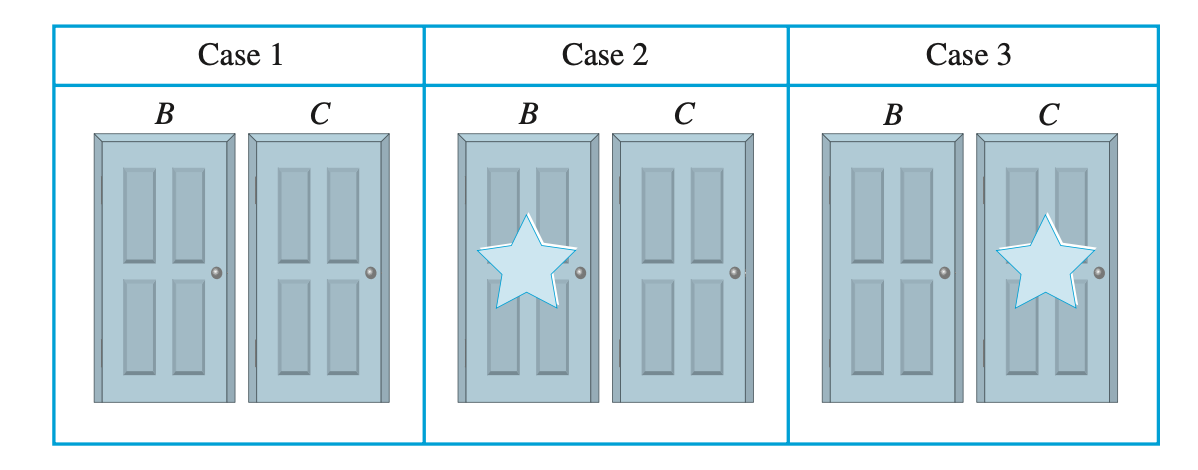
\includegraphics[width=.4\textwidth]{images/monte_hall_solution}
\end{center}

Just before the host opens one of the closed doors, there is no information about the location of the prize. Call the door you pick A.  There are three equally likely possibilities for what lies behind the doors: 
\vspace{-0.2cm}
\begin{itemize}
\item 	(Case 1) The prize is behind A. Here the host could open either door. You would \textbf{win by staying} with your original choice: door A.
\item (Case 2)  The prize is behind B.  Here, the host must open door C, and so you would \textbf{win by switching} to door B.
\item (Case 3)  The prize is behind C.  Here, the host must open door B, and so you would \textbf{win by switching} to door C.
\end{itemize}
%
 Thus, in two of the three equally likely cases, you would win by switching. %from A to the other closed door. %Therefore, you should switch. 
% How to test
\end{frame}

\begin{frame}{A quick conversation with a hypothetical skeptic}

\colorbox{red!30}{Question.} \;  I find both lines of analysis equally compelling! How can I know for sure that the second analysis is the correct one?
\pause 
\vfill \vfill 
\colorbox{green!30}{Answers.}

\begin{enumerate}
	\item \textbf{Mathematical argument.} We can provide a formal mathematical argument using conditional probabilities.  For instance, see pp. 227 of Scheinerman.
	\pause  
	\vfill 
	\item \textbf{Empirical argument.} We can perform repeated experiments (on a computer or in vivo), and find that the number of wins when switching tends towards $\frac{2}{3}$, and the number of wins when staying tends towards $\frac{1}{3}$.
\end{enumerate}

\pause 
\vfill 
\colorbox{yellow!50}{Try it!} \quad 
\scriptsize  \url{https://www.mathwarehouse.com/monty-hall-simulation-online/}

\end{frame}


\begin{frame}[standout]
Group exercises
\end{frame}

\begin{frame}
\footnotesize 
\vfill 
\begin{columns}
\begin{column}{0.33\textwidth}
aaron.loomis: 10 \\ 
adam.wyszynski: 15 \\ 
alexander.goetz: 17 \\ 
alexander.knutson: 7 \\ 
anthony.mann: 20 \\ 
blake.leone: 10 \\ 
bridger.voss: 5 \\ 
caitlin.hermanson: 12 \\ 
cameron.wittrock: 2 \\ 
carsten.brooks: 13 \\ 
carver.wambold: 1 \\ 
colter.huber: 16 \\ 
conner.reed1: 2 \\ 
connor.mizner: 15 \\ 
connor.yetter: 19 \\ 
derek.price4: 16 \\ 
devon.maurer: 7 \\ 
emmeri.grooms: 6 \\ 
erik.moore3: 17 \\ 
ethan.johnson18: 11 \\ 
evan.barth: 8 \\\end{column}
\begin{column}{0.33\textwidth}
evan.schoening: 7 \\ 
griffin.short: 11 \\ 
jack.fry: 20 \\ 
jacob.ketola: 9 \\ 
jacob.ruiz1: 18 \\ 
jacob.shepherd1: 9 \\ 
jada.zorn: 8 \\ 
jakob.kominsky: 16 \\ 
james.brubaker: 9 \\ 
jeremiah.mackey: 20 \\ 
jett.girard: 14 \\ 
john.fotheringham: 21 \\ 
jonas.zeiler: 6 \\ 
joseph.mergenthaler: 13 \\ 
joseph.triem: 12 \\ 
julia.larsen: 5 \\ 
justice.mosso: 19 \\ 
kaden.price: 6 \\ 
lucas.jones6: 3 \\ 
luka.derry: 19 \\ 
luke.donaldson1: 1 \\\end{column}
\begin{column}{0.33\textwidth}
lynsey.read: 13 \\ 
mason.barnocky: 10 \\ 
matthew.nagel: 14 \\ 
micaylyn.parker: 11 \\ 
michael.oswald: 17 \\ 
nolan.scott1: 18 \\ 
owen.obrien: 8 \\ 
pendleton.johnston: 12 \\ 
peter.buckley1: 4 \\ 
reid.pickert: 21 \\ 
ryan.barrett2: 3 \\ 
samuel.hemmen: 18 \\ 
samuel.mosier: 14 \\ 
samuel.rollins: 4 \\ 
sarah.periolat: 4 \\ 
timothy.true: 2 \\ 
tristan.nogacki: 3 \\ 
tyler.broesel: 5 \\ 
william.elder1: 1 \\ 
yebin.wallace: 15 \\ 
zeke.baumann: 21 \\\end{column}
\end{columns}
\vfill
\end{frame}


\begin{frame}{Group exercises}

\begin{enumerate}
	\item Let $(S,P)$ be the sample space with $S=\set{1,2,\hdots, 10}$ and $P(x) =\frac{1}{10}$ for all $x \in S$.  Let $A$ be the event \enquote{is even} and $B$ be the event \enquote{is prime}.  Please calculate the following:
	\vspace{-0.5cm}
    \begin{columnsonlytextwidth}
    \begin{column}[t]{0.22\textwidth}
        \begin{itemize} \small
		\item[a.)] $P(A)$ 
		\item[b.)] $P(B)$
        \end{itemize}
    \end{column}
    \begin{column}[t]{0.22\textwidth}
        \begin{itemize} \small
      	\item[c.)] $P(A \cond B)$
		\item[d.)] $P(B \cond A)$ 
        \end{itemize}
    \end{column}
     \begin{column}[t]{0.22\textwidth}
        \begin{itemize} \small
		\item[e.)] $P(\overline{B} \cond A)$ 
		\item[f.)] $P(B \cond \overline{A})$
        \end{itemize}
    \end{column}
    \begin{column}[t]{0.22\textwidth}
        \begin{itemize} \small
		\item[g.)] $P(\overline{B} \cond \overline{A})$. 
        \end{itemize}
    \end{column}
    \end{columnsonlytextwidth}
    \vspace{.2cm}
     Are the events $A$ and $B$ independent?
\item A card is drawn from a well-shuffled deck of 52-cards.
	\begin{itemize}
	\item[a.] What is the probability that it is a spade ($\spadesuit$)?
	\item[b.] What is the probability that it is a king?	
	\item[c.] What is the probability that it is the king of spades?
	\item[d.] Are the events in parts (a) and (b) independent?
	\end{itemize}
\item Prove Scheinerman Prop. 32.4.
\item Let $A$ and $B$ be events in a sample space with $P(A \cap B) \neq 0$.  Prove that $P(A \cap B) = P(B \cap A)$ if and only if $P(A) = P(B)$.
\end{enumerate}

\end{frame}




\end{document}
